\section{Data storage and management system}

\subsection{The \pd Data Characteristics}
Characteristics of the \pd data are in a large part defined by a few fundamental
properties of the \pd Liquid Argon TPC:
\begin{itemize}
\item The high spatial granularity of the detector (e.g. the pitch of the wires, etc), and the resulting high channel count
\item High digitization frequency (which is essential to ensure a precise position measurement along the drift direction)
\item Relatively slow drift velocity of electrons in Liquid Argon, which  leads to a substantial readout window (of the order of milliseconds) required to collect
all of the ionization in the Liquid Argon volume stemming from the event of interest and overlapping cosmic rays.
\end{itemize}

%\noindent 
Triggered readouts of the detector, denoted ``events'' here, 
thus contain a significant amount of raw data, thus impacting the bandwidth and
storage requirements.   The run plan, which determines the total number of required events, 
helps define the design requirements for the data storage and management system.

The \textit{``\pd/SP Data Scenarios''} spreadsheet\,\cite{data_spreadsheet}  %(DUNE DocDB 1086)
describes three possible running conditions and estimates for their
resulting data volumes and rates and interpretations in terms of
network and disk bandwidth. 
\fixme{Should briefly describe what the 3 running conditions are}
 It also includes estimates for non-beam
data in order to constrain the contributions of cosmic rays to the beam-on data.  Some highlights
of these estimates for the ``most likely'' scenario
are listed in Table~\ref{tab:goldi}. The lossless compression factor cited
in the table is based on the assumption that the signal-to-noise level 
is similar to or better than that achieved by MicroBooNE.

\begin{table}[htbp]
  \centering
  \begin{tabular}[h]{l|r}
\hline
    Trigger rate & \SI{25}{\Hz} \\
    Spill duration & \SI{4.5}{\second} \fixme{should be 4.8s} \\
    SPS Cycle & \SI{22.5}{\second} \\
    Readout time window & \SI{5}{\milli\second} \\
    \# of APAs to be read out & 6 \\
    \hline
    Single readout size (per trigger) & \SI{230.4}{\mega\byte} \\
    Lossless compression factor & 4 \\
    Instantaneous data rate (in-spill) & \SI{1440}{\mega\byte\per\second} \\
    Average data rate & \SI{576}{\mega\byte\per\second} \\
    \hline
    3-Day buffer depth & \SI{300}{\tera\byte} \\
    \hline
  \end{tabular}
  \caption{Parameters defining data rate and volume in the ``most likely'' scenario v5\,\cite{data_spreadsheet}. The buffer depth includes both
  the in-spill and out-of-spill data.}
  \label{tab:goldi}
\end{table}


%The run plan is being finalized at the time of writing. 
\fixme{Check section 7.4 for the run plan and refer to it for any discussion.}
The run plan calls for about 25\,M analyzable beam events to be collected in the first run of \pd. Data sets may be enhanced 
in desirable particle types and energies with dedicated triggers (such as PID) 
from the beam instrumentation. The latter is described in Sec. \ref{beam_instrumentation}. 


Based on a preliminary plan for calibrations which involves measuring a few types of cosmic $\mu$ tracks
(e.g. at different angles, stopped vs not stopped etc),
the current assumption is that for every beam trigger, one non-beam
trigger will be acquired between spills.  Hence, the estimated average data rate and the buffer depth are a factor of two larger,
while the instantaneous data rate remains unchanged.
The setup leads to the requested total samples size of 50\,M events. 

Based on the estimated event readout size quoted in Table\,\ref{tab:goldi}  the anticipated raw data volume 
amounts to about 3\,PB which are to be taken during the planned SPS run.


%%%%%%%%%%%%%%% Tom's stuff
\subsection{Interface of the DAQ to the online storage}
\label{sec:DAQ_online_interface}
% -mxp- commenting out Tom's intro... To save page count
%Just like in many other experiments, the \pd data rate depends on the number of
%triggers needed in order to meet the test and measurement goals, and
%the operating schedule.

%The requirements that the data handling and processing system has to meet are
%determined most  by the desired data rate and, to a lesser extent, the total data volume.
%On the other hand, available funding and personnel place
%constraints on the size and functionality of the online data handling
%and processing system. This makes it necessary to carefully design
%the run program and optimize the system for maximum efficiency and
%performance.


Table\,\ref{tab:goldi} contains the nominal trigger rate of 25\,Hz for
the mid-range scenario. It may be necessary to provide the capability
to run at  an instantaneous trigger rate of up to 100\,Hz in order to
allow for commissioning and schedule delays. For that reason,
scalability of the DAQ, the online buffer and the prompt processing system
\ref{sec:prompt_processing} is an important design requirement.
% the DAQ and online processing system is designed to handle. 
%Up to six APA modules are to be read out on
%each trigger.  The data are assumed to be compressed in the RCE's,
%with a lossless compression ratio of 5.
 Data are assumed to be
collected based on prompt trigger signals generated by the beamline
instrumentation in order to purify samples of desired particles.

The readout of the photon detector channels and the beam
instrumentation is assumed to be a relatively minor addition to the
total data rate and are not anticipated to drive the design of the
data handling and processing system, although adequate resources must
be provisioned in order to acquire and store the data from these
systems.

The network speed of all computers in the data acquisition
chain is anticipated to be 10\,Gbits/sec.  Computers running near-line
processing of subsets of the data, which are generally CPU-bound, may
be connected with 1\,GBit/sec links.  The software framework for
interfacing with the electronics, building events, writing data files,
and providing an interface to online monitoring of data as it is
acquired is {\it artdaq}~\cite{artdaq}.

Assuming that each RCE reads out 256 channels of the TPC, 60 RCE's
will need to be active.  Ten computers running BoardReader
processes will read out six RCE's each.  These computers should be
provisioned with at least 8 cores and 16 GBytes of RAM each, along
with a 10\,Gbit/sec network connection.  The BoardReader processes will
transmit data to a set of computers running EventBuilder processes.
A number of Event Builder computers (netween 10 and 20), each with 8 cores and 16\,GB of RAM
and a 10\,Gbit/sec NIC will provide the CPU and networking needed to
build events, collectbasic metadata, optionally perform basic online monitoring,
and send the data to storage.  The Event Builders assemble data fragments sent by the
BoardReaders into self-consistent events consisting of readout data
from each contributing RCE, SSP, and beam instrumentation information
for the same time period.  They will also perform basic data integrity
checks, ensuring that all data that are expected for an event have
arrived and have not been corrupted, before writing records out.

The online buffer layer will consist of $\sim$300\,TB of high-speed disks, which may be connected directly to the Event Builders
or accessbile via the network.  As of this writing, three approaches are being considered:
\begin{itemize}
\item a XRootD cluster~\cite{xrootd} taking data directly from the Event Builders over the network.

\item high-speed storage devices (SSD) attached to the Event Builders, forming a moderate-capacity buffer;
an external storage cluster will still be needed in order to satisfy the nominal 3-day buffer capacity requirement.

\item a commercial-grade NAS with adequate capacity and network bandwidth.

\end{itemize}

\noindent Each version has its advantages and disadvantages. Technology choice will be made after
additional R\&D and testing.

%A alternative to this design that allows for more flexibility but at a
%cost of network latency and CPU, is to add a layer of Aggregator CPU
%processes between the EventBuilders and the disk writing.  These
%processes may be needed if the events are to be sorted, analyzed,
%reformatted, or otherwise handled before writing out.  In order to
%maximize throughput and minimize cost, the number of steps in the data
%handling system is to be minimized.

After the data are written to disk by {\it artdaq}, the data handling
system creates metadata files,optionally  runs near-line monitoring jobs, and
transfers the data from EHN1 to the CERN Computing Centre, as
described in DUNE DocDB~1212~\cite{docdb1212}. According to the current plan,
the ``F-FTS'' software developed and maintained at FNAL will be the central element
of the data flow management at this level.


\subsection{Raw Data Flow in \pd}
\label{sec:raw_concept}
%%%%%%%%%%%%%%%%%%%%%%%%
\begin{figure}[tbh]
\centering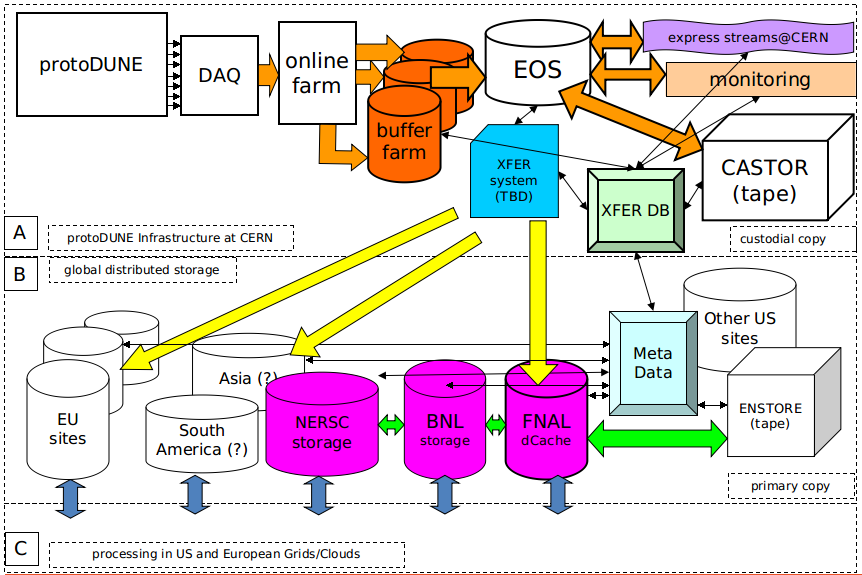
\includegraphics[width=\linewidth]{protoDUNE_raw_data_concept.png}
\caption{\label{fig:raw_concept}Conceptual diagram of the flow of raw data in \pd}
\end{figure}
%%%%%%%%%%%%%%%%%%%%%%%%

\noindent
Conceptual diagram of the raw data flow in \pd is presented in Fig.\ref{fig:raw_concept}. It shows the general logic
of data flow, and does not include specific assumptions about what system will be used to actually move the data.
It also reflects the central role of CERN EOS in the \pd raw data management scheme. This is motivated by the experience
and architecture of the LHC experiments.

EOS serves as the staging area from which the data gets committed to CASTOR
and from which it is transmitted to a number of endpoints including principal data centers such as FNAL and others.
It is also used to provide input to QA and other express processing streams at CERN (sec.\,\ref{sec:prompt_processing}).
%This scheme assumes that there is no conceptual difference between NP02 and NP04 in terms of the general pattern of data flow.

Data centers at BNL and NERSC are placed in this diagram for illustration purposes. Any other institution possessing adequate
resources can participate in this data distriburtion scheme if desired. According to the design presented in DUNE DocDB~1212~\cite{docdb1212}
this part of the data transmission process is also handled by an instance of F-FTS.


